\documentclass[12pt]{article}
\usepackage{a4wide}
\usepackage{amsmath,amssymb}
\usepackage{bm}
\usepackage[colorlinks]{hyperref}
\usepackage{graphicx}

\usepackage{algorithm}
\usepackage{algorithmic}

\usepackage{float}
\usepackage{bbold}
\usepackage{comment}
\usepackage{mathtools}


%\usepackage{caption,refstyle}

% Package diagramme Processus de Production de la GS
\usepackage{tikz}
\usetikzlibrary{positioning, shadows}


\usepackage[french]{babel}
\usepackage[T1]{fontenc}
\usepackage{lmodern}

\DeclareUnicodeCharacter{2009}{\,} 
\usepackage[standard]{ntheorem}



\usepackage{tikz}
\usepackage{graphicx}
\usetikzlibrary{positioning, arrows.meta}
\usepackage{amsmath}
\usepackage{pdfpages}
\usepackage{adjustbox}




\begin{document}

\begin{titlepage}
\title{}
\author{Congo Job
\\ Stage Master 2 \\
 IRMA, Université de Strasbourg, France}
\date{ }

\begin{figure}[b!]
\centering
\vfill
\includegraphics[scale=0.16]{Images/logo-unistra.pdf}
\hspace{0.5 cm}
\includegraphics[scale=0.16]{Images/logo-Fonderie.pdf}
\hspace{0.5 cm}
\includegraphics[scale=0.16]{Images/logoCSMI.pdf}
\end{figure}
\end{titlepage}


\maketitle
\thispagestyle{empty}


\newpage

\tableofcontents

\newpage

% \section{Présentation de l'entreprise : Fonderie de Niederbronn}
\section{Contexte }


%  Mettre une introduction générale ici soit en section soit sans!!!
\subsection{Introduction rapide}


% Dire quelque généralité

La fonderie est un secteur qui fabrique des pièces moulées en métal. 
Elle couvre une variété d’alliages, du fer à l’aluminium en passant 
par le cuivre.

Dans ce document, nous avons le rapport de stage qui a eu lieu dans l'équipe
d'Informatique de la Fonderie de Niederbronn. Il s'est déroulé sur
une période de quatre mois, entre le 11 mars et le 26 juillet 2024. 
On retrouvera tous les documents du stage dans ce 
lien : \url{https://github.com/master-csmi/2022-stage-job-br}. 


% Presenter rapidement le plan du rapport
Le présent rapport couvre les éléments suivants : la présentation de 
la fonderie de Niederbronn, la description du processus 
de production et de l'objectif du stage, l'étude statistique,  

mandat du stage la méthodologie utilisée durant le stage, et les résultats du stage. En
fin une conclusion boucle ce rapport de stage.



\subsection{Présentation de la Fonderie de Niederbronn}

%---- presenter la Fonderie,...

La Fonderie de Niederbronn, fondée en 1769, est un partenaire clé dans la production de pièces 
en fonte. Grâce à son expérience et son savoir-faire, l'entreprise produit des pièces en fonte 
à graphite lamellaire (GJL) et à graphite sphéroïdal (GJS) pour une clientèle industrielle variée,
aussi bien en France qu'à l'international. L’usine est située au Nord-Est de la France 
à Niederbronn près de Strasbourg.



\subsubsection*{Capacités et Installations de Production}
\textbf{Moyens de Fusion:}
\begin{itemize}
    \item 2 fours Junker 5T d'une puissance de 4MW.
\end{itemize}

\textbf{Lignes de Moulage:}
\begin{itemize}
    \item \textbf{DISAMATIC 270} : Coulée automatique verticale pour des pièces jusqu'à 950 x 700 mm et un poids maximum de 40 kg.
    \item \textbf{HWS} : Coulée automatique horizontale pour des pièces de dimensions jusqu'à 1600 x 1400 mm et un poids maximum de 600 kg.
\end{itemize}

\textbf{Moyens de Noyautage:}
\begin{itemize}
    \item 5 machines à noyer avec une capacité de production allant de 1 à 100 litres et des noyaux jusqu'à 300 kg.
\end{itemize}

\textbf{Moyens de Peinture:}
\begin{itemize}
    \item 2 lignes de peinture liquide pouvant traiter des pièces jusqu'à 500 kg. Peintures disponibles : primaire d'accrochage, peinture résistante aux brouillards salins de 300h, haute température (600°C).
\end{itemize}

\textbf{Moyens d'Usinage:}
\begin{itemize}
    \item Tours et centres d'usinage CNC avec des capacités variées pour des pièces de grandes dimensions (jusqu'à 1200 x 1000 x 600 mm).
\end{itemize}

\subsubsection*{Contrôle Qualité}
La Fonderie de Niederbronn attache une grande importance à la qualité de ses produits, mise en œuvre à travers divers contrôles :
\begin{itemize}
    \item \textbf{Dimensionnel:} Utilisation de bras FARO et scan 3D.
    \item \textbf{Non Destructif:} Banc de magnétoscopie et contrôle par ultrasons.
    \item \textbf{Caractéristiques Mécaniques:} Traction, contrôle de dureté, résilience.
    \item \textbf{Métallurgiques:} Spectrométrie et micrographie.
\end{itemize}

\subsubsection*{Secteurs d'Activité}
\sloppy
La Fonderie de Niederbronn sert plusieurs secteurs industriels et domestiques, 
en fournissant des pièces spécifiques adaptées aux besoins de chaque domaine.
\begin{itemize}
    \item \textbf{Usage Industriel :} Le Machinisme Agricole, les Machines du BTP, les Pièces Hydrauliques,...
    \item \textbf{Usage Domestique :} Les Corps de Chaudière et Radiateurs, les Poêles et Inserts de Cheminée,...
\end{itemize}

\subsubsection*{Chiffres Clés et Ressources Humaines}
\begin{itemize}
    \item \textbf{Nombre de Collaborateurs:} 170.
    \item \textbf{Capacité de Fusion:} 20 000 tonnes par an.
    \item \textbf{Chiffre d'Affaires:} 23 millions d'euros pour l'exercice 2023.
\end{itemize}


% - Mettre les 2 images fonderie vue de haut et une autre en vue de face.
\sloppy
Cette présentation met en lumière l'expertise, les capacités de production,
et l'engagement qualité de la Fonderie de Niederbronn, faisant d'elle un acteur 
incontournable dans le secteur de la fonderie.


\begin{figure}[H]
    \centering
    \vfill
    \includegraphics[scale=0.27]{Images/Fonderie_vue_de_bas.pdf}
    \hspace{0.5 cm}
    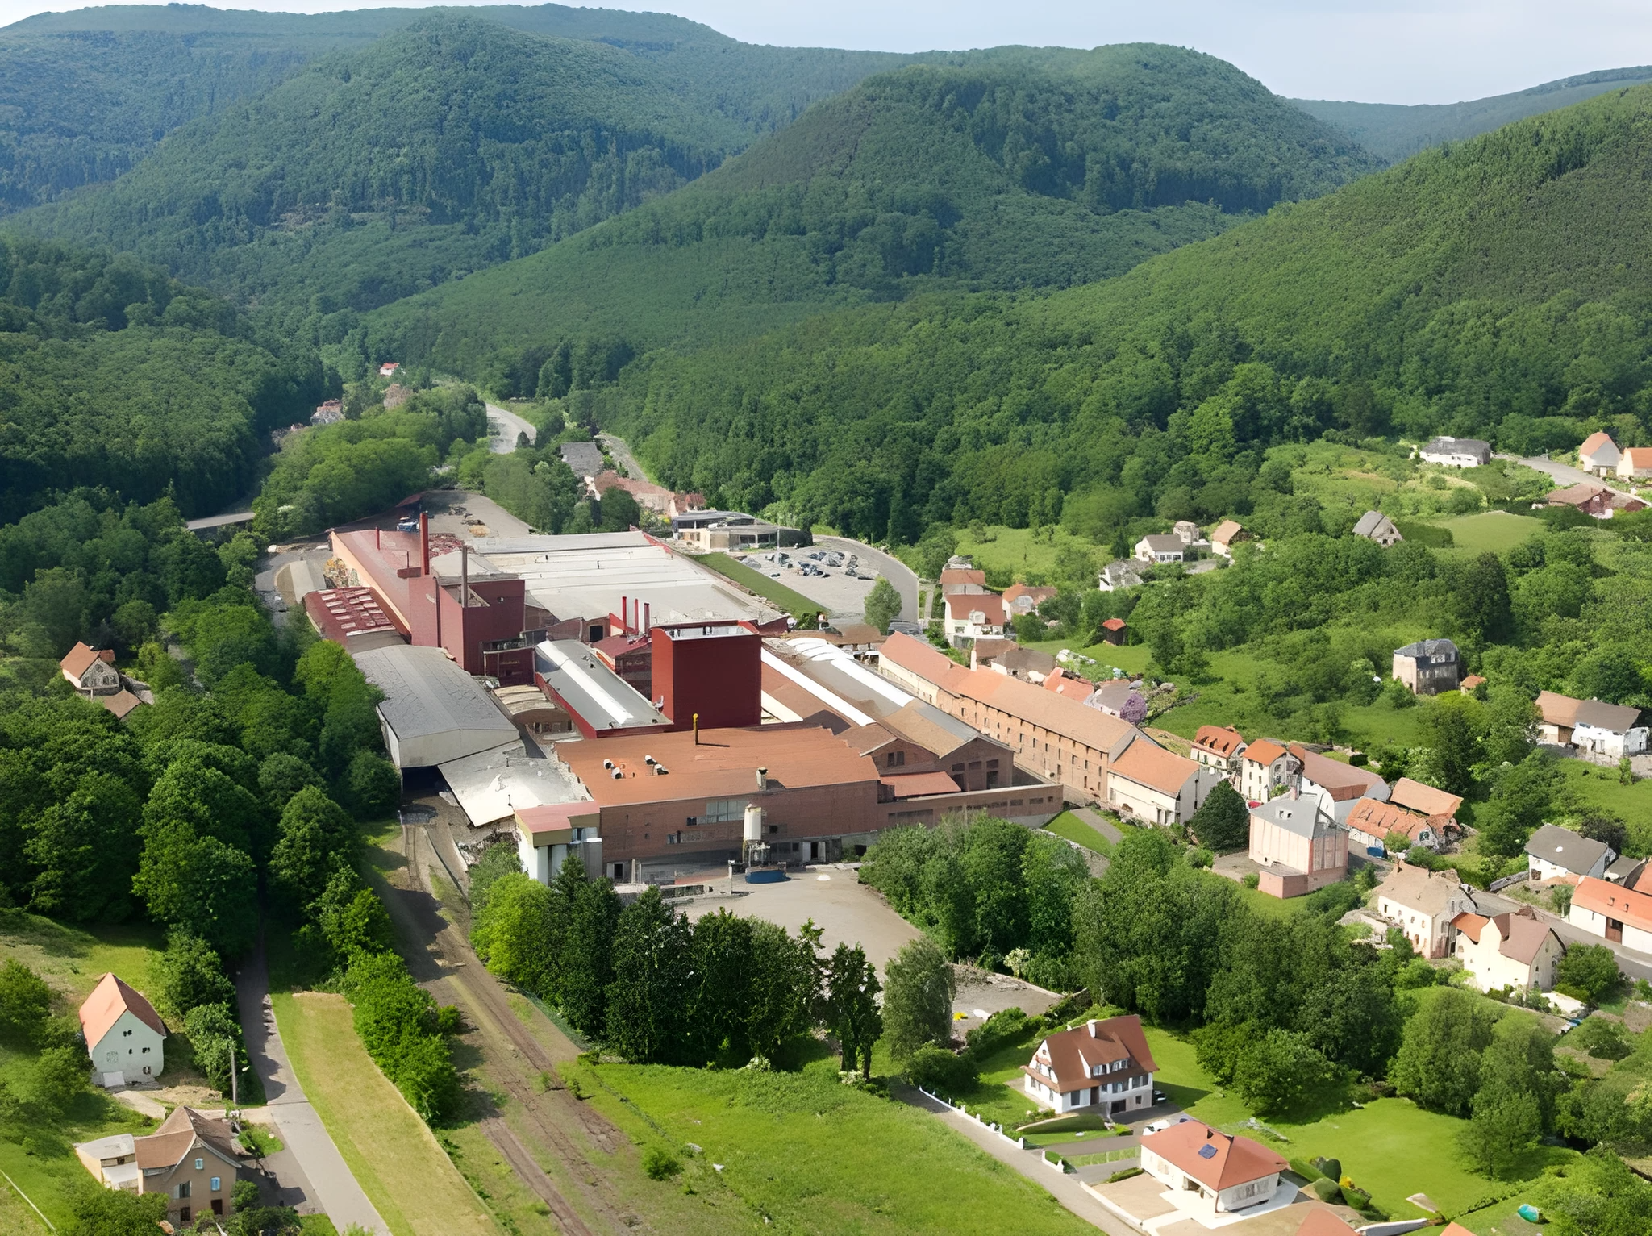
\includegraphics[scale=0.27]{Images/Fonderie_vue_de_haut.pdf}
    \caption{Vues extérieure et aérienne de la Fonderie de Niederbronn}
\end{figure}

\newpage

\subsection{Description du processus de production des pièces en fonte}

Voici un schéma décrivant les différents étapes de production d'une pièce en fonte :


% 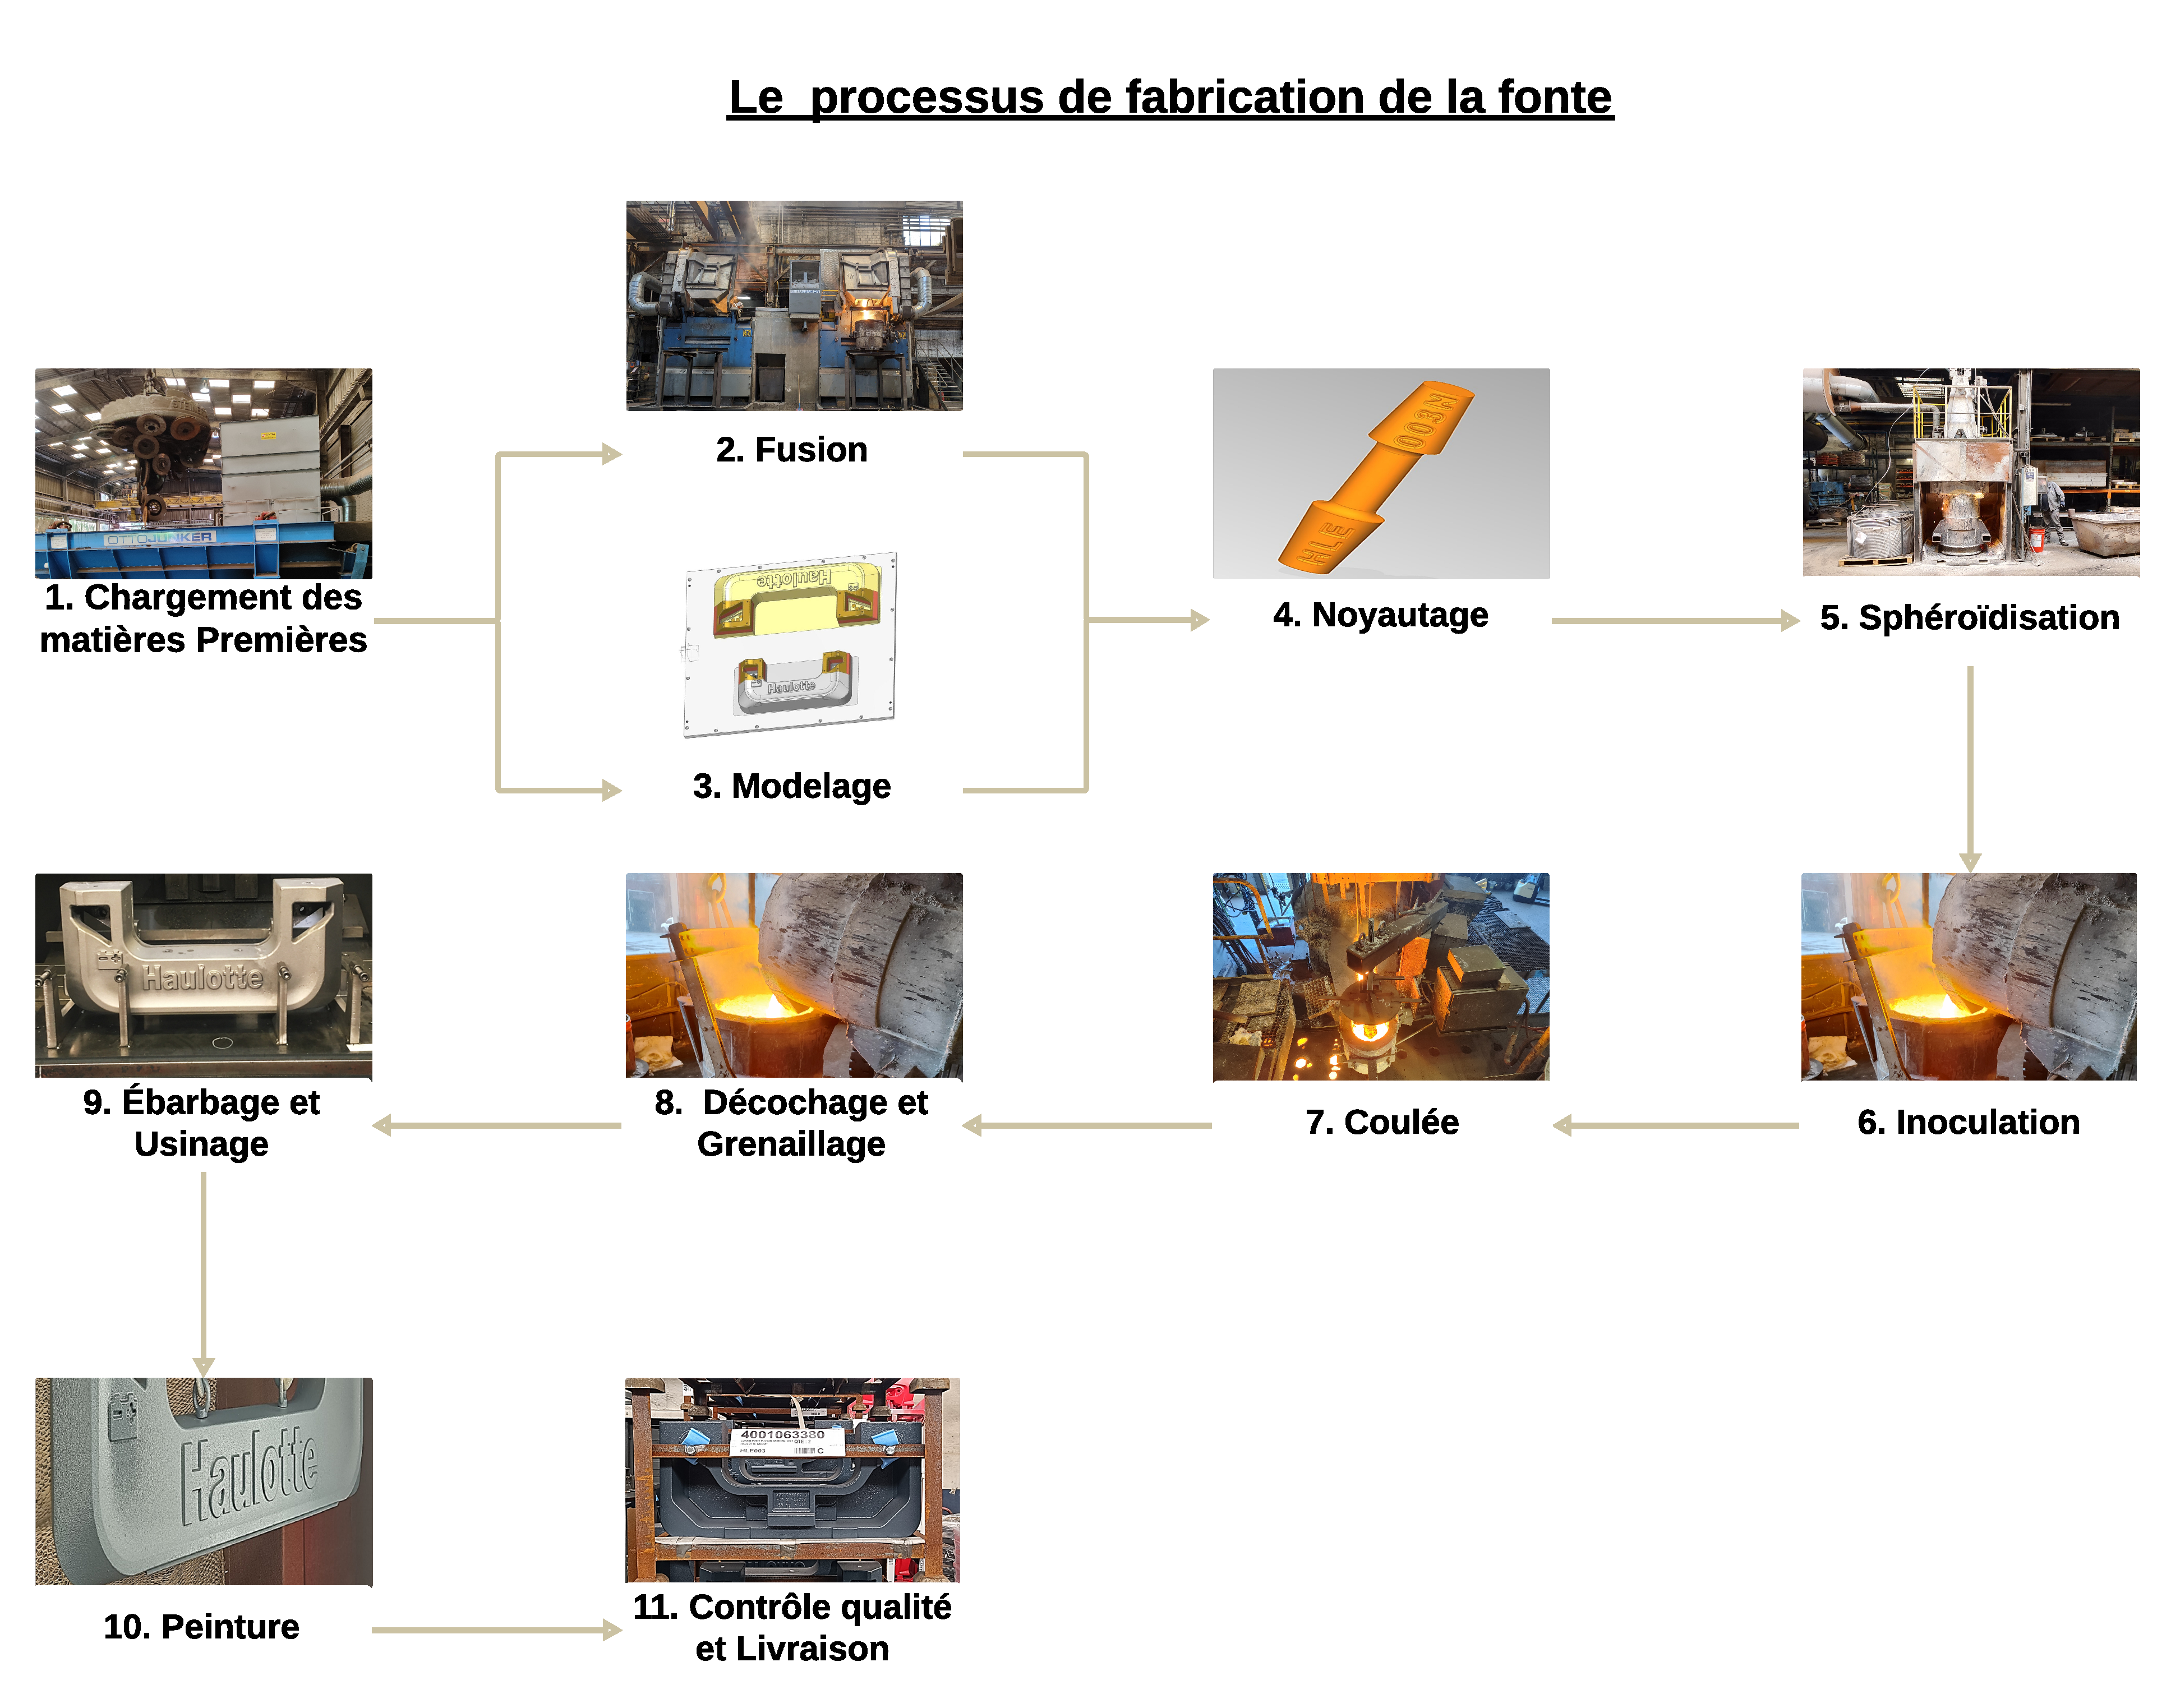
\includepdf[pages=-, scale=1]{Images/Flux de production.pdf}

\begin{figure}[H]
    \centering
    \begin{adjustbox}{width=1.3\textwidth,height=0.8\textheight,center}
        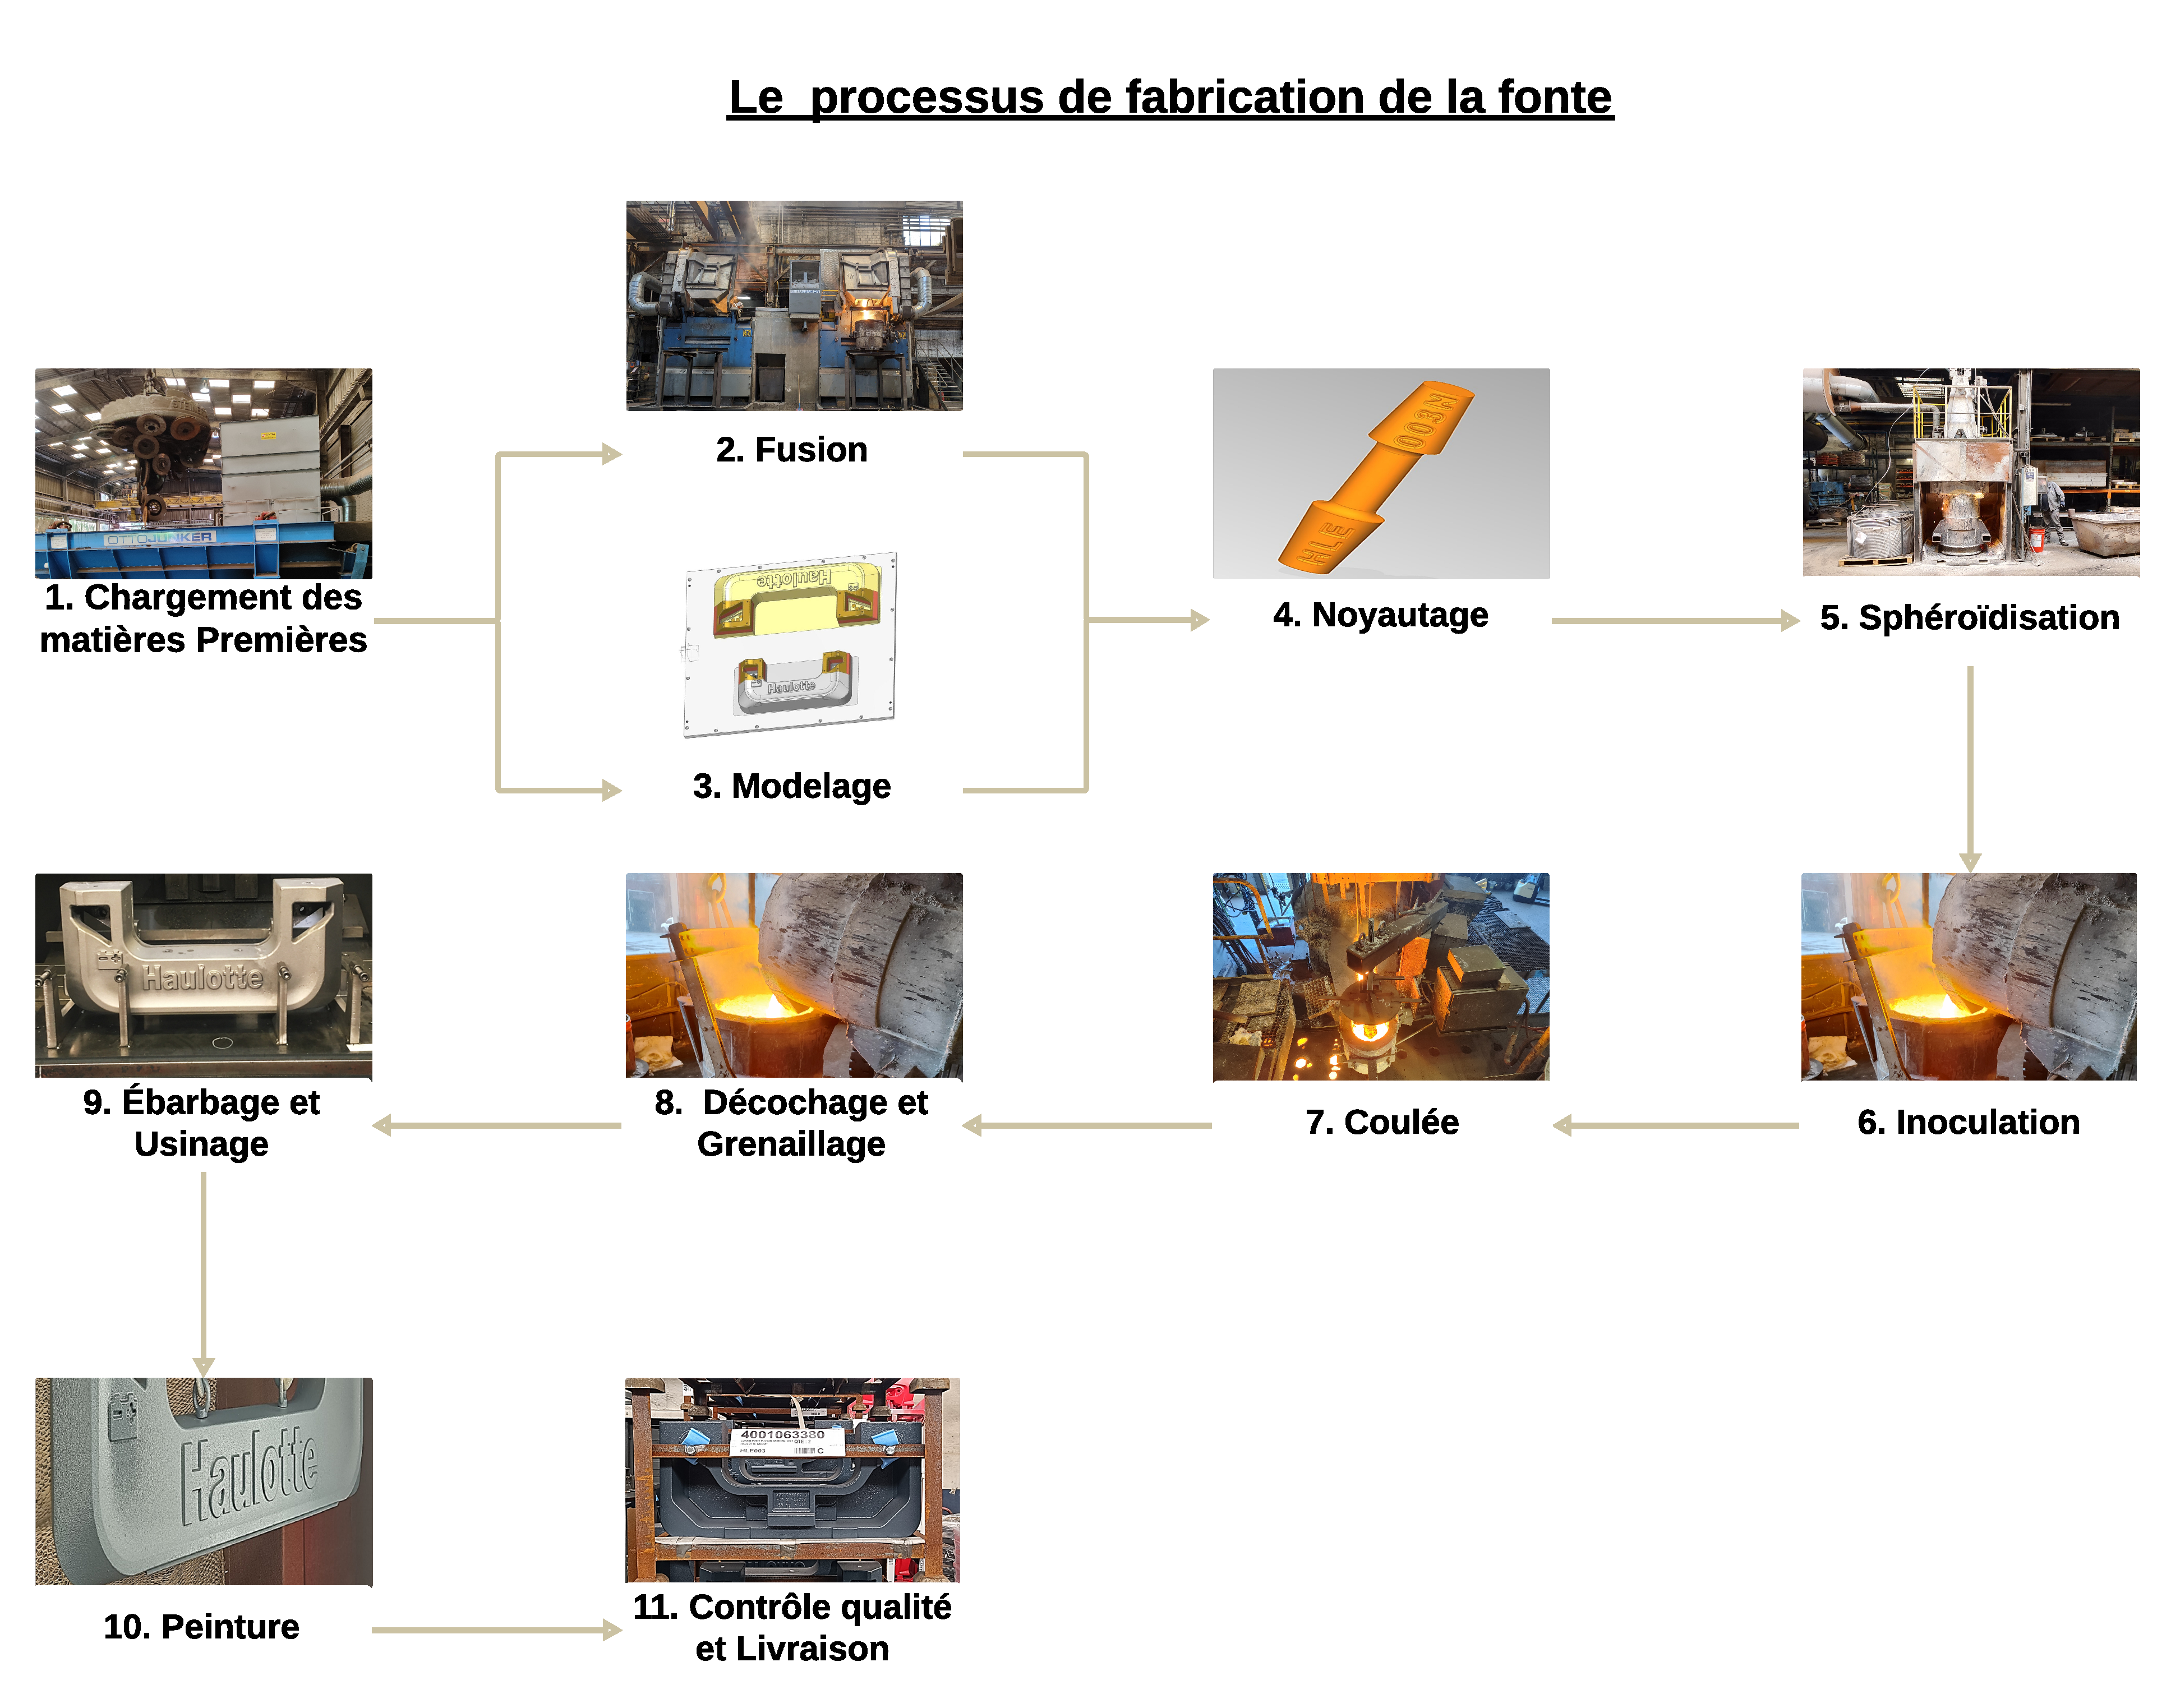
\includegraphics{Images/Flux de production.pdf}
    \end{adjustbox}
    \caption{Flux de production des pièces en fonte.}
    \label{fig:flux-production}
\end{figure}


\begin{enumerate}
    \item \textbf{Chargement des matières premières :}
    Dans cette étape, les matériaux de base nécessaires pour la production de la 
    fonte sont préparés. Cela inclut la sélection, le tri et le nettoyage des 
    matières premières telles que le ferraille, le coke, le calcaire, et les alliages
    nécessaires (comme le magnésium et le silicium). La composition précise de ces 
    matériaux est cruciale pour obtenir les propriétés mécaniques désirées dans la 
    fonte.

    % ----------------- Mettre image des matières premières

    \item \textbf{Fusion :} Le matériau préparé est fondu dans un four à haute 
    température pour le rendre liquide. Cette fusion est essentielle pour permettre 
    le moulage ultérieur du matériau. Le métal est fondu dans un four à induction à 
    haute température. 



    \item \textbf{Modélage :} 
    La première étape dans la production en fonderie est la préparation du 
    modèle et du moule. Le modèle est une réplique de la pièce finale, 
    généralement réalisée en bois, en plastique ou en métal. 
    Le moule est fabriqué en utilisant le modèle pour créer une cavité 
    dans laquelle le métal en fusion sera coulé. Il existe plusieurs types 
    de moules, mais les plus courants sont les moules en sable.

    Les ingénieurs conçoivent le modèle en utilisant des logiciels de CAO 
(Conception Assistée par Ordinateur) pour s'assurer que la pièce finale 
respectera les spécifications demandées. Cette étape inclut :

\begin{itemize}
    \item Analyse des besoins du client et des spécifications techniques.
    \item Création du modèle 3D à l'aide de logiciels spécialisés comme SolidWorks ou CATIA.
    \item Validation du modèle avec des simulations numériques pour anticiper les contraintes et les défauts potentiels.
\end{itemize}


Le modèle est fabriqué à partir de matériaux spécifiques en fonction de 
la complexité et des exigences de la pièce finale. Les matériaux couramment 
utilisés incluent :

\begin{itemize}
    \item Bois pour des pièces uniques ou de grande taille.
    \item Plastique pour des productions en série grâce à des techniques comme l'impression 3D.
    \item Métal pour des modèles de haute précision ou des moules permanents.
\end{itemize}


Le modèle est ensuite utilisé pour créer le moule. Pour les moules en sable,
un mélange de sable et de liant est compacté autour du modèle pour créer 
une cavité exacte de la pièce à produire. Cette étape comprend :

\begin{itemize}
    \item Préparation du sable en ajustant la granulométrie et en ajoutant des liants.
    \item Compactage du sable autour du modèle dans un cadre ou une boîte de moulage.
    \item Séparation du modèle du moule sans détériorer la cavité.
    \item Assemblage des parties du moule et des canaux de coulée pour guider le métal liquide.
\end{itemize}


    \item \textbf{Noyautage :} 


    \item \textbf{Sphéroïdisation :} Après la fusion, la fonte liquide est traitée 
    pour favoriser la formation de sphéroïdes de graphite. Ce processus implique 
    l'ajout de magnésium sous forme d'alliage. Le magnésium réagit avec le fer fondu 
    pour former des sphéroïdes de graphite, ce qui améliore la ductilité et la 
    résistance de la fonte. Les pourcentages précis de magnésium ajoutés et les 
    rendements de l'opération sont calculés pour garantir une formation optimale 
    des sphéroïdes.
    % ----------------- Mettre image Microscopique de la fonte GS
    \item \textbf{Inoculation et Dégrassage :} Dans cette étape, des agents d'inoculation sont 
    ajoutés au métal fondu pour contrôler la structure et les propriétés finales de 
    la fonte GS. Ces agents favorisent la formation de sphéroïdes de graphite de 
    taille et de forme uniformes.

    L'inoculation est réalisée après la sphéroïdisation pour contrôler la structure 
    et les propriétés finales de la fonte. Des agents inoculants, tels que le 
    ferrosilicium, sont ajoutés pour favoriser une précipitation uniforme et fine 
    du graphite. Comme mentionné dans l'image GS 3, les taux d'addition et les 
    conditions d'inoculation sont optimisés pour obtenir la structure souhaitée. 
    Cela inclut des considérations sur la teneur en calcium et en silicium.

    % ----------------- Mettre image Innoculation/Degrassange en action ou du produits innoculant
    \item \textbf{Moulage ou Coulée :} Le métal fondu est versé dans des moules qui ont la 
    forme et les dimensions souhaitées pour les pièces finales. Le processus de 
    moulage peut être effectué selon différentes techniques, telles que le moulage 
    au sable ou le moulage sous pression, en fonction des exigences spécifiques du 
    produit.


    Une fois fondu, le métal est versé dans le moule à travers un système de canaux appelés « systèmes de coulée ». Le métal liquide remplit la cavité du moule et prend la forme du modèle. Cette étape nécessite une attention particulière pour :

\begin{itemize}
    \item Contrôler la température du métal pour éviter des défauts comme les inclusions ou les porosités.
    \item Utiliser des techniques de dégazage pour éliminer les gaz dissous dans le métal.
    \item Assurer un remplissage uniforme et éviter les turbulences qui pourraient introduire des impuretés.
\end{itemize}

    \item \textbf{Décochage et Grenaillage :} 

    Après la coulée, le métal liquide doit refroidir et se solidifier pour prendre la forme finale de la pièce. Le temps de refroidissement varie en fonction du type de métal et de la taille de la pièce.

    Un refroidissement contrôlé est essentiel pour éviter les défauts dans la pièce finale. Des systèmes de refroidissement peuvent être utilisés pour réguler la température, comme :

    \begin{itemize}
        \item L'utilisation de noyaux refroidisseurs en métal ou en céramique.
        \item L'application de traitements thermiques pendant le refroidissement pour modifier la structure du métal.
        \item La mise en place de systèmes de refroidissement à eau ou à air pour des pièces de grande taille.
    \end{itemize}

    
    Une fois le métal solidifié, le moule est cassé ou retiré pour récupérer la pièce. Pour les moules en sable, le moule est détruit pour libérer la pièce coulée. Cette étape peut inclure :

\begin{itemize}
    \item Le cassage manuel ou mécanique du moule.
    \item Le nettoyage de la pièce pour enlever les résidus de sable ou de liant.
    \item L'inspection initiale de la pièce pour détecter des défauts majeurs.
\end{itemize}

    \item \textbf{Ebarbage et Usinage :} 
    La pièce obtenue après démoulage n'est pas encore prête pour une utilisation directe. Elle doit subir plusieurs opérations de finition et une inspection de qualité rigoureuse.
    Les excédents de métal et les bavures sont enlevés par des opérations de meulage ou de découpage. Cela inclut :

    
    \item \textbf{Peinture :} 

    \item \textbf{Contrôle qualité et Livraison :} Avant la livraison des pièces finales, un 
    contrôle qualité est effectué pour s'assurer qu'elles répondent aux normes et 
    aux spécifications requises. Cela peut inclure des tests de dimension, de 
    résistance, de ductilité, ainsi que des inspections visuelles et des tests non 
    destructifs. Une fois les pièces passées avec succès les contrôles 
    qualité, elles sont prêtes à être livrées au client ou au processus suivant dans 
    la chaîne de production. Cette étape marque la conclusion du processus de 
    production de la fonte GS.

    La pièce est inspectée pour détecter tout défaut interne ou externe. Les méthodes d'inspection incluent :

\begin{itemize}
    \item La radiographie, pour détecter les défauts internes comme les fissures ou les inclusions.
    \item Les ultrasons, pour examiner l'intégrité interne sans détruire la pièce.
    \item Les tests de dureté, pour vérifier que les propriétés mécaniques sont conformes aux spécifications.
    \item Les contrôles dimensionnels, pour s'assurer que les dimensions respectent les tolérances définies.
\end{itemize}
\end{enumerate}


    % \item  \textbf{Conclusion:} Le processus de production en fonderie est complexe et implique plusieurs étapes cruciales pour garantir la qualité et la précision des pièces fabriquées. Chaque étape, de la conception du modèle à l'inspection finale, doit être réalisée avec précision pour répondre aux exigences spécifiques du client. La maîtrise de ces processus est essentielle pour l'efficacité et la compétitivité de l'entreprise dans le secteur de la fonderie. En conclusion, une compréhension approfondie et une exécution rigoureuse de chaque phase du processus de production sont indispensables pour produire des pièces de haute qualité et satisfaire les besoins du marché.





\subsection{L'objectif du stage }


% Presenter rapidement L'objectif du stage
L’objectif principal de ce stage est d’optimiser l’utilisation des matières 
premières recyclées dans la production de fonte à hautes caractéristiques 
mécaniques. Le projet s’inscrit dans le cadre d’un crédit d’impôt recherche 
et vise à modéliser et automatiser les processus liés au choix et aux 
quantités des différentes matières premières. Voici les missions confiées :

\begin{itemize}
    \item Modéliser le système via des équations.
    \item Contribuer à l’optimisation des coûts de revient en 
    automatisant les processus.
    \item Participer à d’autres sujets d’optimisation en parallèle.
\end{itemize}





\subsection{Le plan du rapport}

% Presenter rapidement le plan du rapport
Le présent rapport couvre les éléments suivants : la présentation de 
la fonderie de Niederbronn, la description du processus 
de production et de l'objectif du stage, 

mandat du stage la méthodologie utilisée durant le stage, et les résultats du stage. En
fin une conclusion boucle ce rapport de stage.



%---- motiver le sujet et objectif stage



%---- détail objectif stage


\subsection{Plan du rapport }

\begin{table}[H]
    \caption{Tableau 1.5: Composition chimique des fontes GS (ADI) [26]}
    \centering
        \begin{tabular}{|c|c|}
        \hline
        Nuance & Carbone [\%] \\ \hline
        GS 400-15 & 3.50-4.00  \\ \hline
        GS 450-10 & 3.50-4.00  \\ \hline
        \end{tabular}
\end{table}
    
    
% \begin{table}[H]
% \caption{Tableau 1.5: composition chimique des fontes GS (ADI) [26]}
%     \begin{tabular}{|l|l|l|l|l|l|l|}
%     \hline
%     Nuance & Carbone (\%) & Silicium (\%) & Manganèse (\%) & Phosphore (\%) & Soufre (\%) & Magnésium (\%) & Cuivre (\%) \\ \hline
%     FGS400-15 & 3.50-4.00 & 2.50-2.80 & <0.30 & 4.30-4.95 & <0.06 & <0.20 \\ \hline
%     FGS450-10 & 3.50-4.00 & 2.50-2.88 & <0.45 & 4.30-4.90 & <0.06 & <0.20 \\ \hline
%     \end{tabular}
% \end{table}


\section{Etude statistique }

\subsection{Présentation du problème d'Optimisation }



\section{La recette Optimale}

\subsection{Présentation du problème d'Optimisation }

Dans le cadre du processus de fabrication de 5 tonnes de fontes, l'une des étapes préliminaires fondamentales
réside dans la détermination du lit de fusion, c'est-à-dire la proportion des matières premières
nécessaires à la fusion. Dans notre cas, on souhaite  produire une tonne de fonte de haute qualité.
Pour ce faire, nous disposons d'une trentaine de matières premières, chacune possédant sa propre
composition chimique distinctive. Chaque matière première est disponible ou non en quantité limitée
et leurs prix varient tout au long de l'année. Ces matières sont issues de diverses sources,
comprenant des matériaux métalliques et de construction, ainsi que des retours, c'est-à-dire
des résidus provenant des précédents cycles de production. Par exemple, parmi ces matériaux,
on trouve les SABOTS DE FREINS SNCF, les RAILS DE CHEMIN DE FER de 40 cm et de la FONTE GS RECYCLÉE,
dont les prix respectifs sont de 435 euros, 423,90 euros et 374 euros. La qualité de la fonte dépend
de sa composition chimique, qui doit se situer dans des intervalles spécifiques adaptés au type
de fonte recherché, tout en respectant des critères de qualité tels que le niveau d'impuretés et
la pureté ONO. Le niveau d'impuretés et la pureté ONO sont déterminés par des combinaisons linéaires
des pourcentages d'éléments chimiques présents dans les matières premières. Par conséquent,
l'objectif principal est de déterminer les proportions optimales des matières premières,
en vue de minimiser les coûts de production tout en préservant la qualité de la fonte.

% (Afficher les images de matières premières de la fonderie)

\subsection{Modélisation du problème}



Phase Tansitoire 

- Explication de cette phase 


- Obtention des images inputs, outpouts Optimisation de la Presentations
Dans le drive , exporter en pdf avec parametre Paysage, Statement, dessus puis bas


Les différents étapes  de la poche 1


\includepdf[pages=-, scale=1]{Images/Poche 1.pdf}
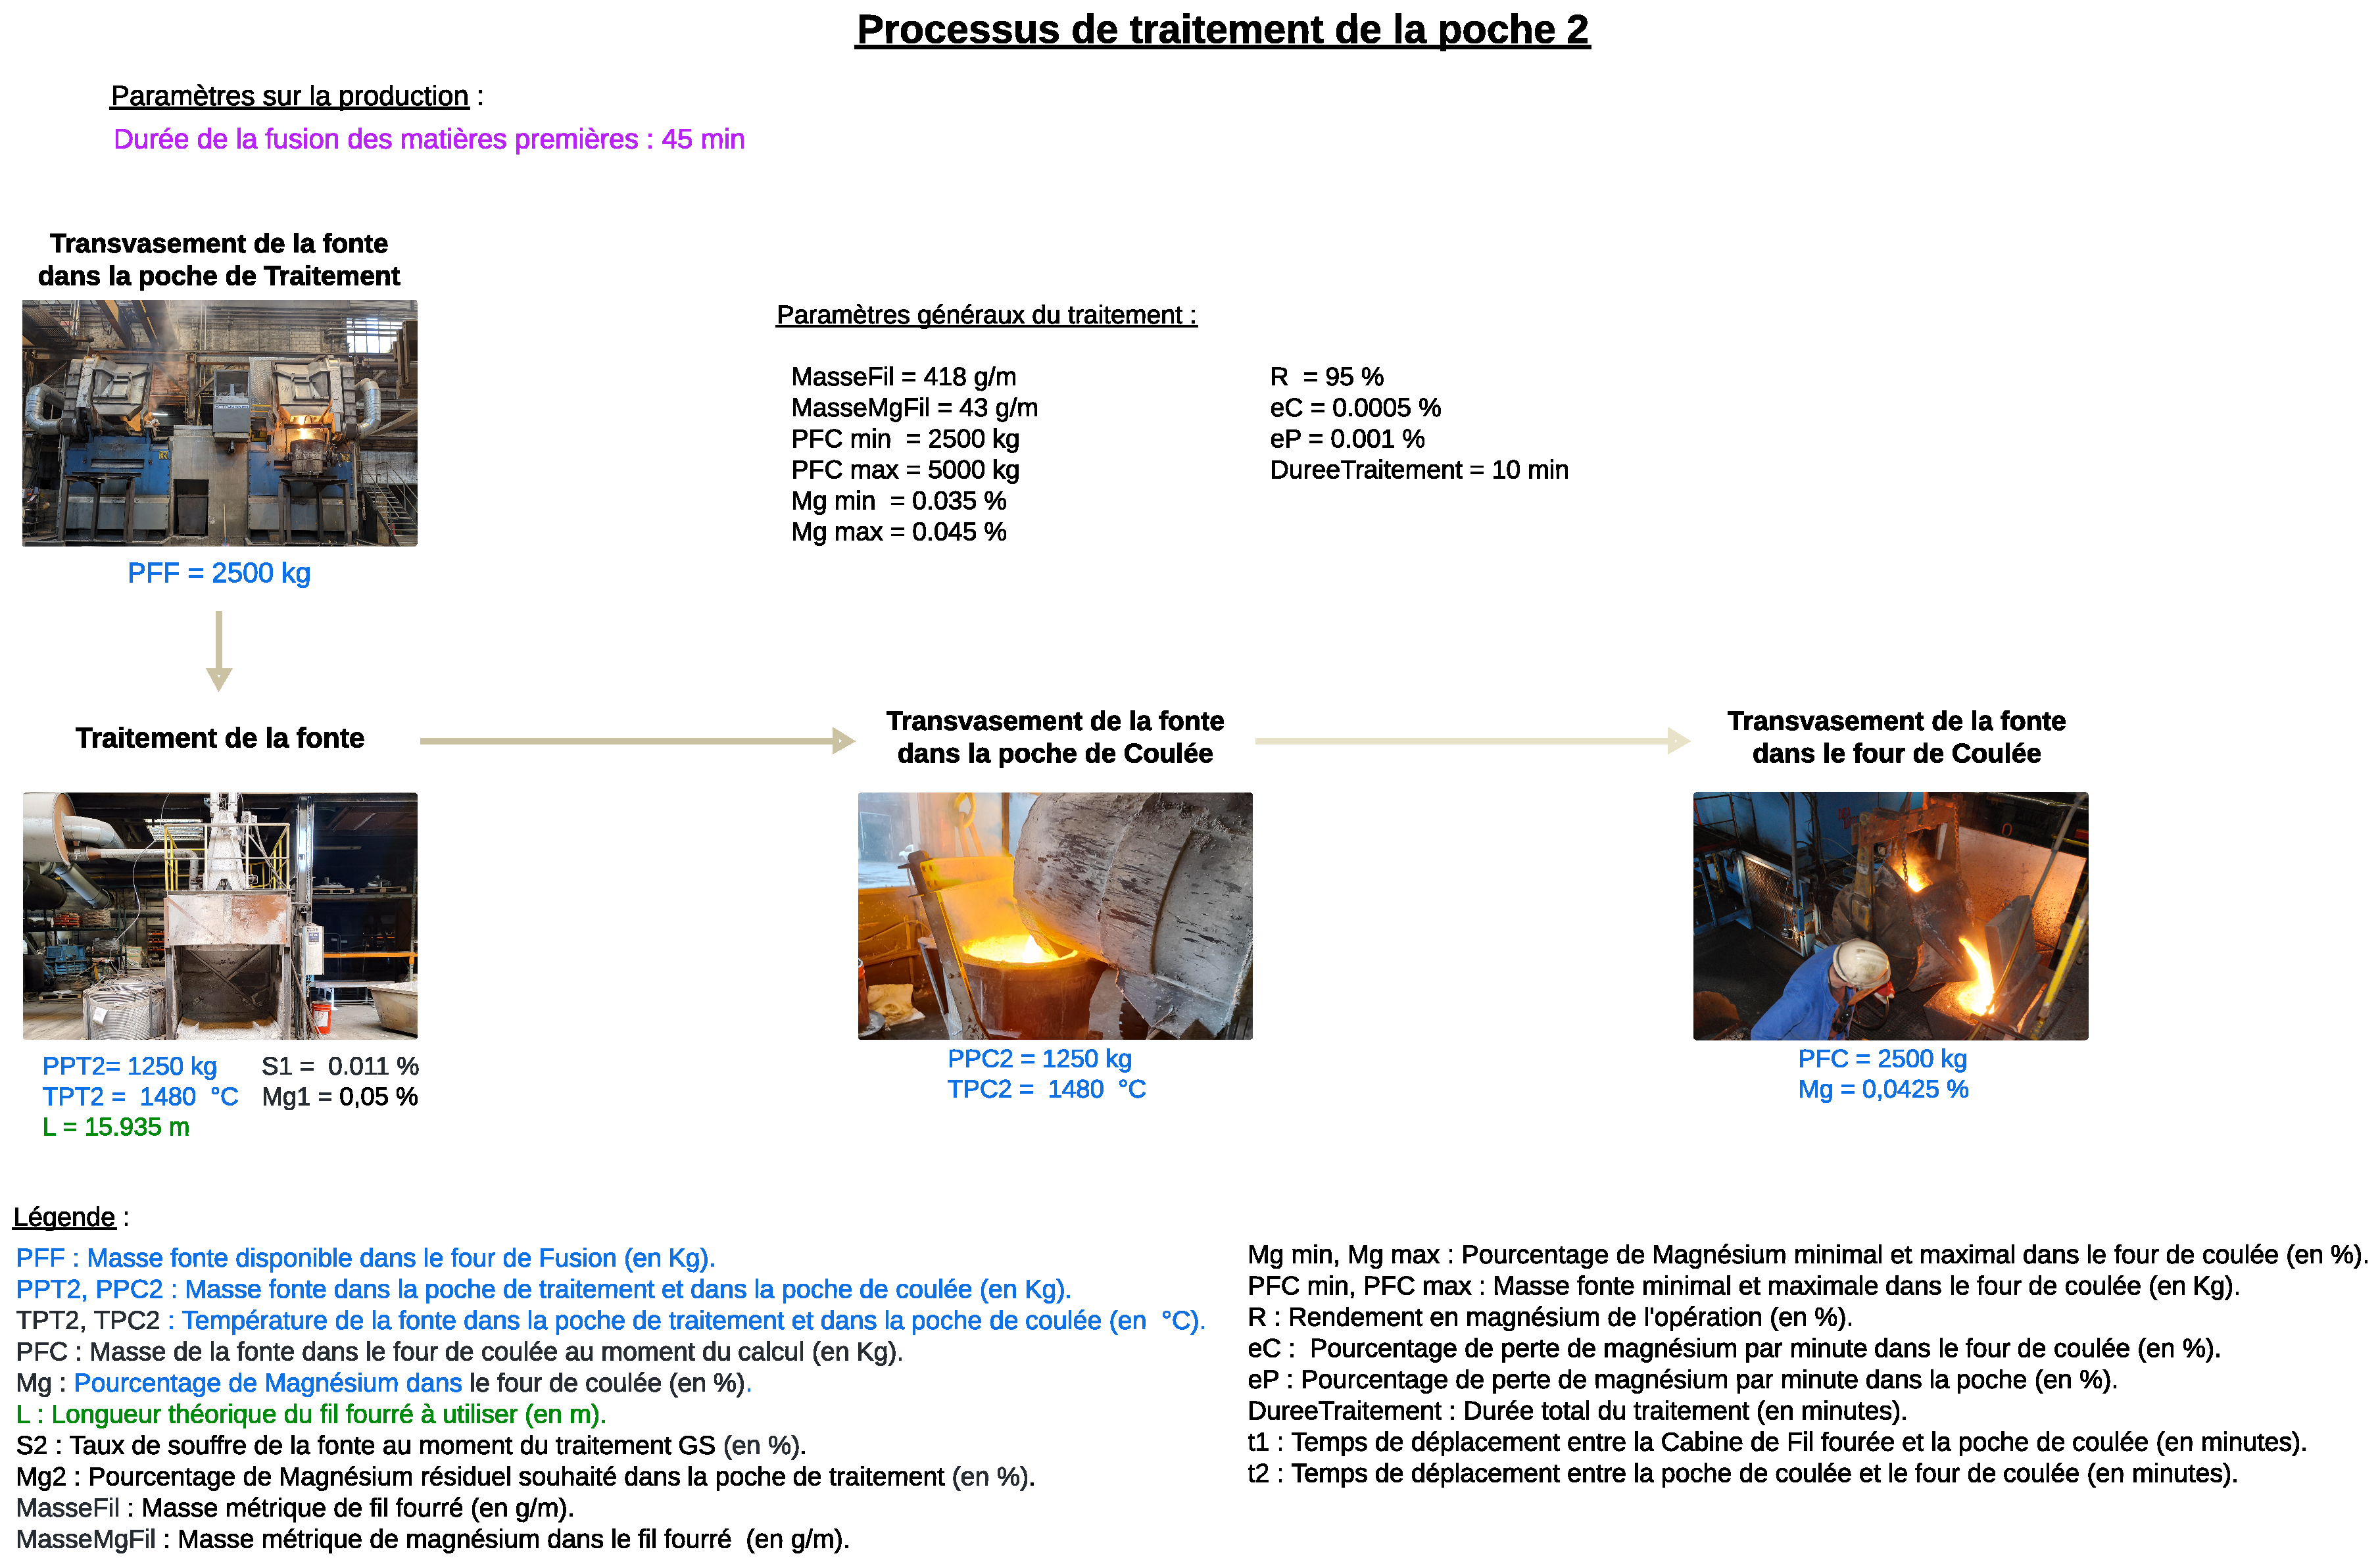
\includepdf[pages=-, scale=1]{Images/Poche 2.pdf}
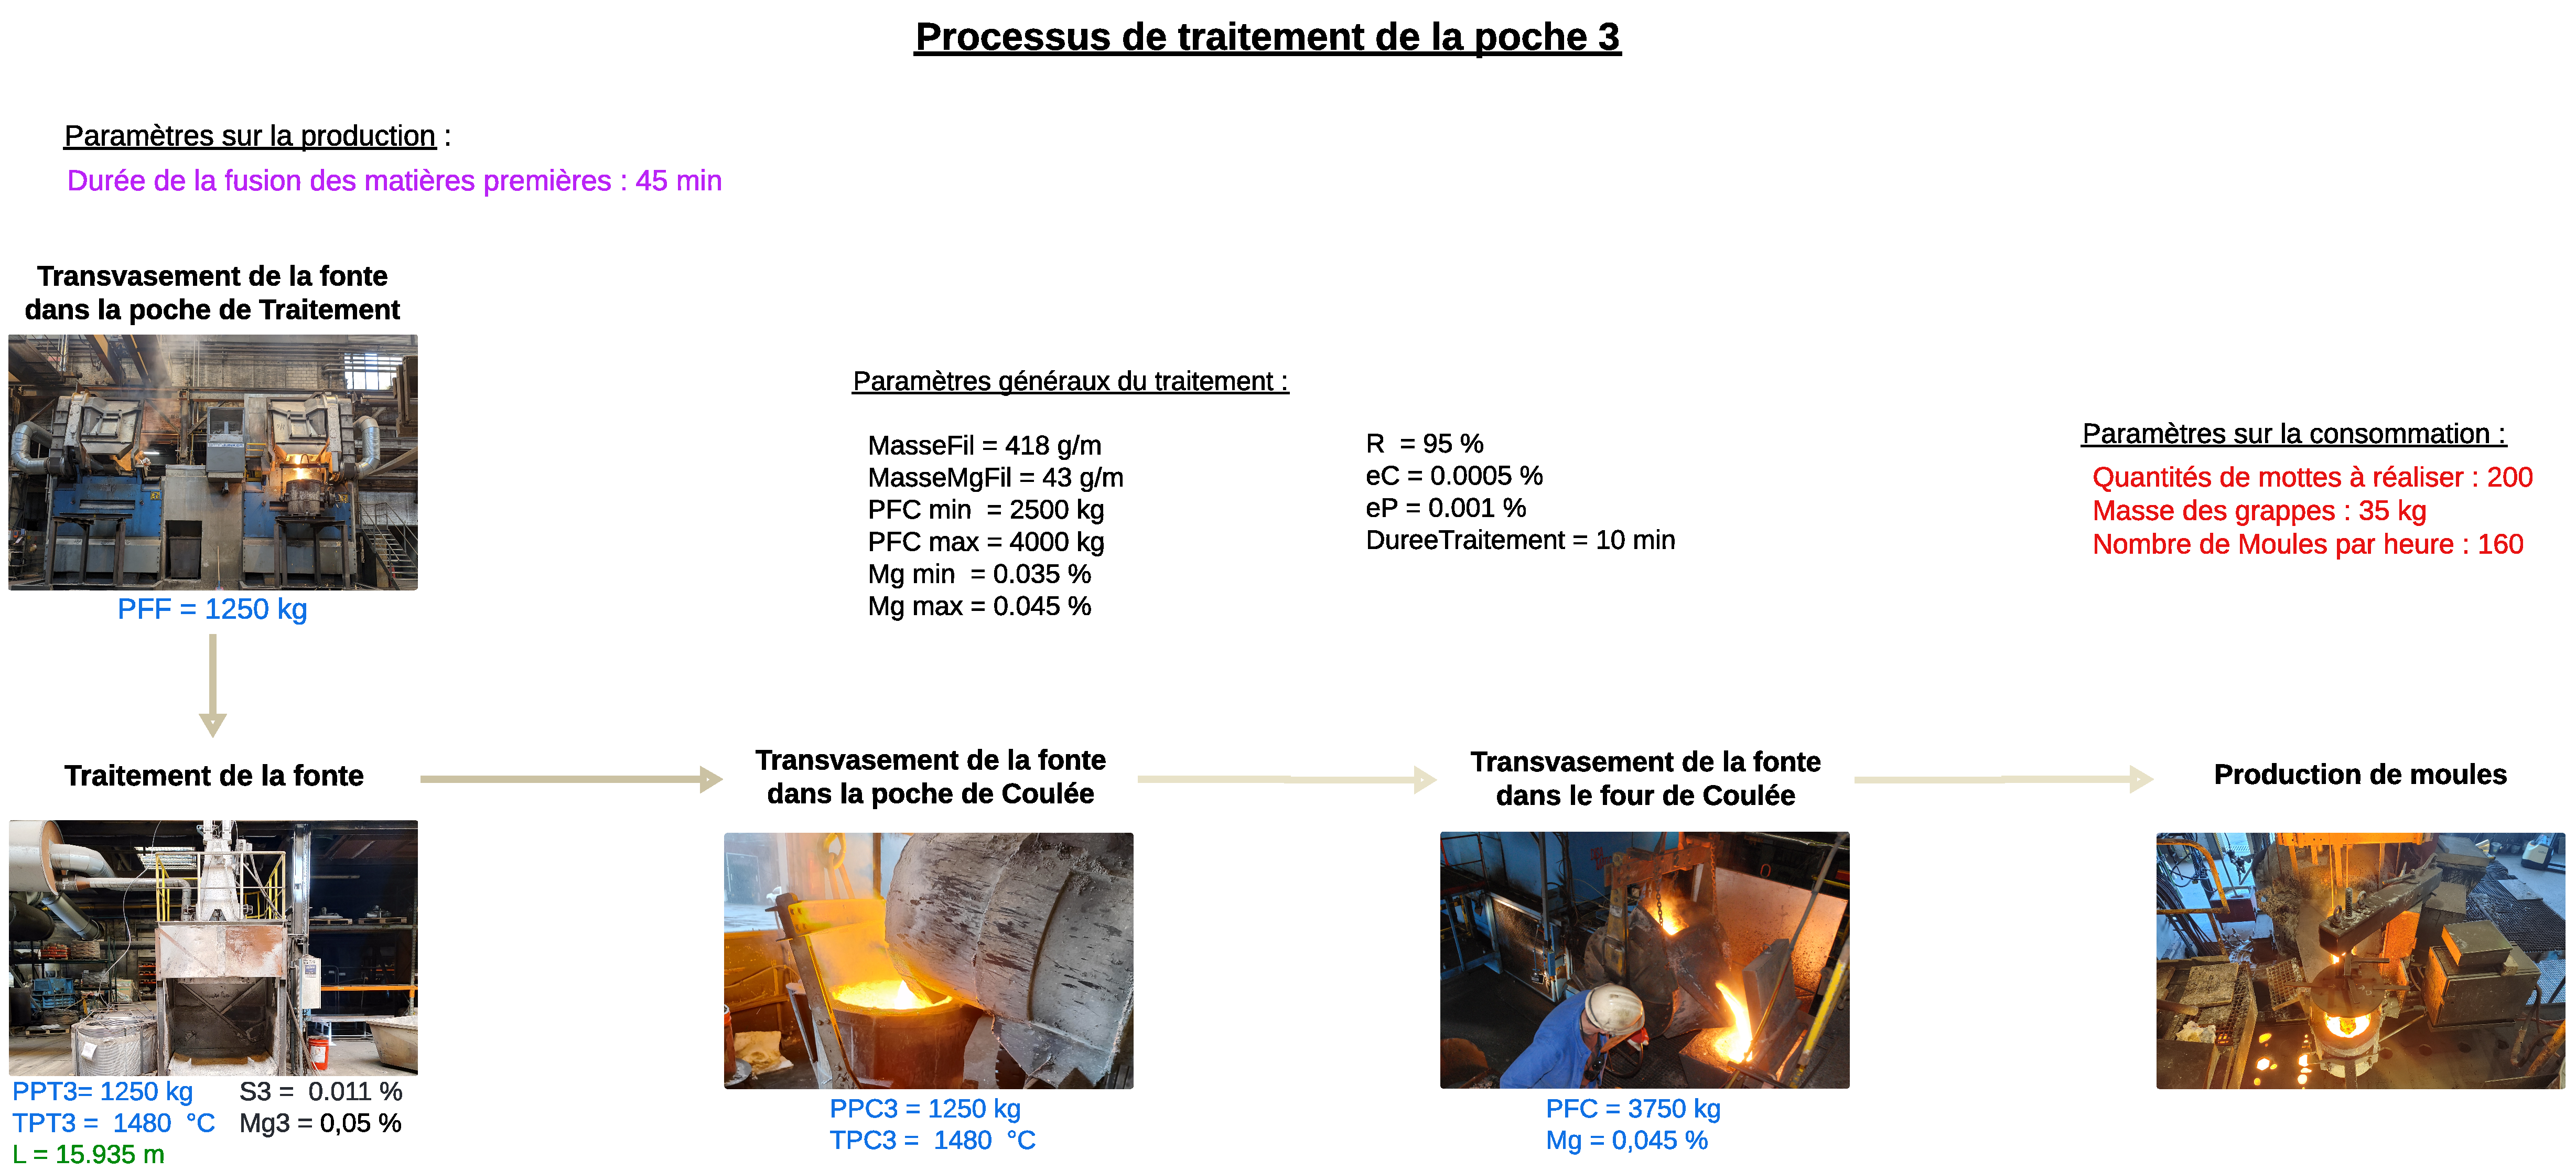
\includepdf[pages=-, scale=1]{Images/Poche 3.pdf}



\subsection{La méthode du simplexe}

\subsection{Mise en oeuvre de la méthode du simplexe}




\begin{thebibliography}{9}

\bibitem{Gianluigi Rozza}
Gianluigi Rozza.  \emph{An introduction to reduced basis method for parametrized PDEs, ResearchGate}

\bibitem{B. Haasdonk}
B. Haasdonk.  \emph{Reduced Basis Methods for Parametrized PDEs –
A Tutorial Introduction for Stationary and
Instationary Problems, University of Stuttgart  } 


\bibitem{Alexandre Ern}

\bibitem{Bopeng RAO}
Bopeng RAO,  \emph{ Méthodes Numériques
des Equations aux Dérivées Partielles. UFR de Mathématique et d’Informatique
Université de Strasbourg, 2021-2022 }

\bibitem{Gwenol Grandperrin}
Gwenol Grandperrin.  \emph{Introduction à la méthode des bases réduites, ResearchGate Janvier 2008 }

\end{thebibliography}

\end{document}